\section{Convolutional Neural Networks for Dense Image Labeling}
\label{sec:convnets}

%\subsection{Model Architecture and Training}
%\label{sec:convnet-arch}

Herein we describe how we have re-purposed and finetuned the publicly
available Imagenet-pretrained state-of-art 16-layer classification network of
\cite{simonyan2014very} (VGG-16) into an efficient and effective dense feature
extractor for our dense semantic image segmentation system.

\subsection{Efficient Dense Sliding Window Feature Extraction with the Hole Algorithm}
\label{sec:convnet-hole}

Dense spatial score evaluation is instrumental in the success of our dense CNN
feature extractor. As a first step to implement this, we convert the
fully-connected layers of VGG-16 into convolutional ones and run the network
in a convolutional fashion on the image at its original resolution. However
this is not enough as it yields very sparsely computed detection scores (with
a stride of 32 pixels). To compute scores more densely at our target stride of
8 pixels, we develop a variation of the method previously employed by
\citet{GCMG+13, sermanet2013overfeat}. We skip subsampling after the last two
max-pooling layers in the network of \citet{simonyan2014very} and modify the
convolutional filters in the layers that follow them by introducing zeros to
increase their length (\by{2}{} in the last three convolutional layers and
\by{4}{} in the first fully connected layer). We can implement this more
efficiently by keeping the filters intact and instead sparsely sample the
feature maps on which they are applied on using a stride of 2 or 4 pixels,
respectively. This approach is known as the `hole algorithm' (`atrous
algorithm') and has been developed before for efficient computation of the
undecimated wavelet transform \cite{Mall99}. We have implemented this within
the Caffe framework \citep{jia2014caffe} by adding to the \textsl{im2col}
function (it converts multi-channel feature maps to vectorized patches) the
option to sparsely sample the underlying feature map. This approach is
generally applicable and allows us to efficiently compute dense CNN feature
maps at any target subsampling rate without introducing any approximations.

We finetune the model weights of the Imagenet-pretrained VGG-16 network to
adapt it to the image classification task in a straightforward fashion,
following the procedure of \citet{long2014fully}. We replace the 1000-way
Imagenet classifier in the last layer of VGG-16 with a 21-way one. Our loss
function is the sum of cross-entropy terms for each spatial position in the
CNN output map (subsampled by 8 compared to the original image). All positions
and labels are equally weighted in the overall loss function. Our targets are
the ground truth labels (subsampled by 8). We optimize the objective function
with respect to the weights at all network layers by the standard SGD
procedure of \citet{KrizhevskyNIPS2013}.

During testing, we need class score maps at the original image resolution. As
illustrated in Figure~\ref{fig:score-maps} and further elaborated in
Section~\ref{sec:local-chal}, the class score maps (corresponding to
log-probabilities) are quite smooth, which allows us to use simple bilinear
interpolation to increase their resolution by a factor of 8 at a negligible
computational cost. Note that the method of \citet{long2014fully} does not use
the hole algorithm and produces very coarse scores (subsampled by a factor of
32) at the CNN output. This forced them to use learned upsampling layers,
significantly increasing the complexity and training time of their system:
Fine-tuning our network on PASCAL VOC 2012 takes about 10 hours, while
they report a training time of several days (both timings on a modern GPU).

\subsection{Shrinking the Receptive Field and Accelerating Dense Computation
  with Convolutional Nets}
\label{sec:convnet-field}

Another key ingredient in re-purposing our network for dense score computation
is explicitly controlling the network's receptive field size. Most recent
DCNN-based image recognition methods rely on networks pre-trained on the
Imagenet large-scale classification task. These networks typically have large
receptive field size: in the case of the VGG-16 net we consider, its receptive
field is \by{224}{224} (with zero-padding) and \by{404}{404} pixels if the net
is applied convolutionally. We consider this receptive field size to be too
large to allow good localization accuracy (unless one uses heavily zoomed-in
versions of the image). Moreover, after converting the network to a fully
convolutional one, the first fully connected layer has 4,096 filters of large
\by{7}{7} spatial size and becomes the computational bottleneck in our dense
score map computation.

We have addressed both of these serious practical problems by spatially
subsampling the first FC layer to \by{4}{4} spatial size. This has reduced the
receptive field of the network down to \by{128}{128} (with zero-padding) or
\by{308}{308}) (in convolutional mode) and has reduced computation time for
the first FC layer by 3 times. Using our Caffe-based implementation and a
Titan GPU, the resulting VGG-derived network is very efficient: Given a
\by{306}{306} input image, it produces \by{39}{39} dense raw feature scores at
the top of the network at a rate of about 8 frames/sec during testing. The
speed during training is 3 frames/sec. Using smaller networks such as
\citet{KrizhevskyNIPS2013} could allow video-rate test-time dense feature
computation even on light-weight GPUs.

\section{Detailed Boundary Recovery: Fully-Connected Conditional Random Fields and Multi-scale Prediction}
\label{sec:boundary-recovery}

\subsection{Deep Convolutional Networks and the Localization Challenge}
\label{sec:local-chal}

As illustrated in Figure~\ref{fig:score-maps}, DCNN score maps can
reliably predict the presense and rough position of objects in an image but
are less well suited for pin-pointing their exact outline. There is a natural
trade-off between classification accuracy and localization accuracy with
convolutional networks: Deeper models with multiple max-pooling layers have
proven most successful in classification tasks, however their increased
invariance and large receptive fields make the problem of inferring position
from the scores at their top output levels more challenging.

The reduced receptive field size in our network architecture can ameliorate
but not fully resolve this problem. Recent work has pursued two directions to
address this localization challenge. The first approach is to harness
information from multiple layers in the convolutional network in order to
better estimate the object boundaries \citep{long2014fully, eigen2014predicting}. The second approach is
to employ a super-pixel representation, essentially delegating the
localization task to a low-level segmentation method. This route is followed
by the very successful recent method of \citet{mostajabi2014feedforward}.

In Section~\ref{sec:dense-crf}, we pursue a novel alternative direction based
on coupling the recognition capacity of DCNNs and the fine-grained
localization accuracy of fully connected CRFs and show that it is remarkably
successful in addressing the localication challenge, producing accurate
semantic segmentation results and recovering object boundaries at a level of
detail that is well beyond the reach of existing methods.  

%We have also
%pursued a hybrid approach in which we combine the proposed fully-connected CRF
%method with our own variant of multi-scale prediction. This combined approach
%yields a further performance improvement, as discussed in
%Section~\ref{sec:multiscale}.

\subsection{Fully-Connected Conditional Random Fields for Accurate Localization}
\label{sec:dense-crf}

\begin{figure}[ht]
  \centering
  \begin{tabular}{c c c c c}
    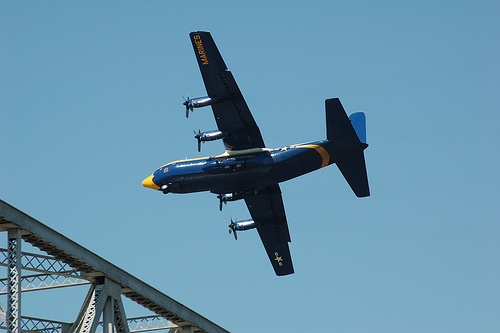
\includegraphics[width=0.16\linewidth]{fig/mean_field_illustration/2007_007470.jpg} & 
    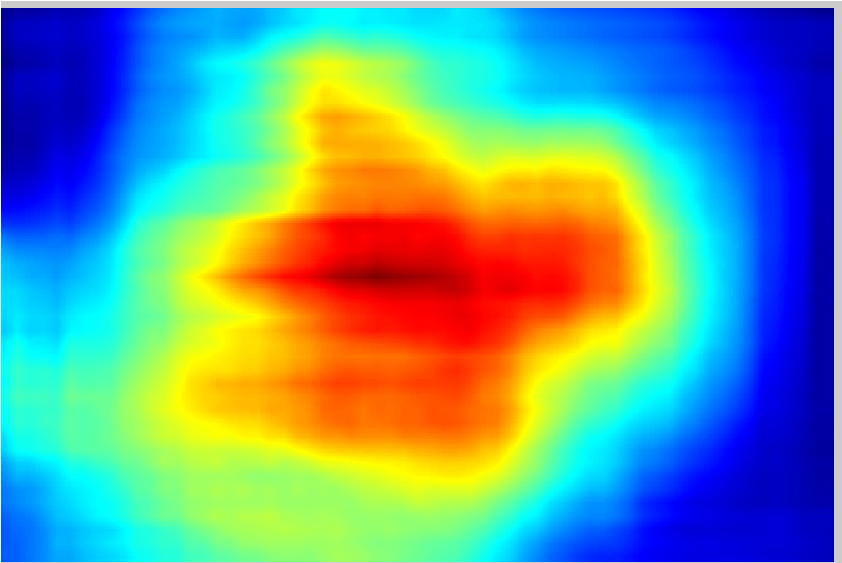
\includegraphics[width=0.16\linewidth]{fig/mean_field_illustration/Score_Class1_Itr0.pdf} &
    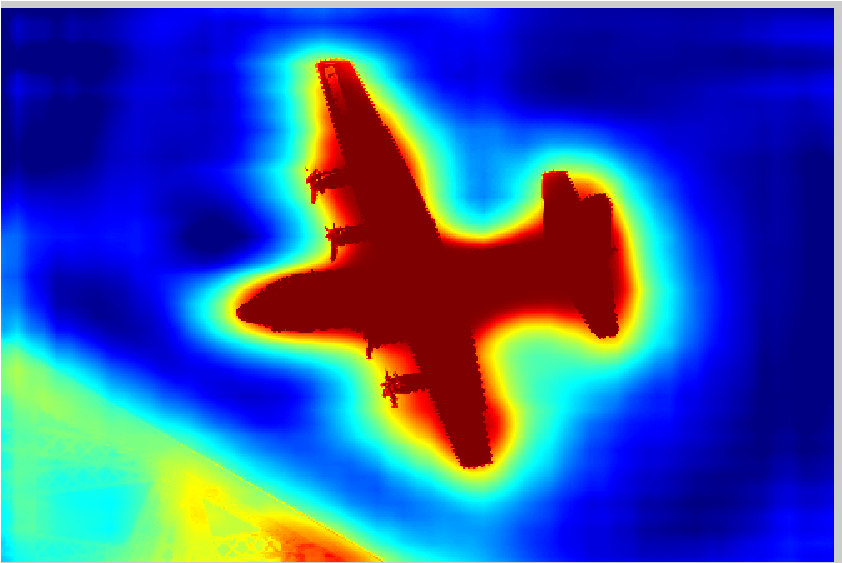
\includegraphics[width=0.16\linewidth]{fig/mean_field_illustration/Score_Class1_Itr1.pdf} & 
    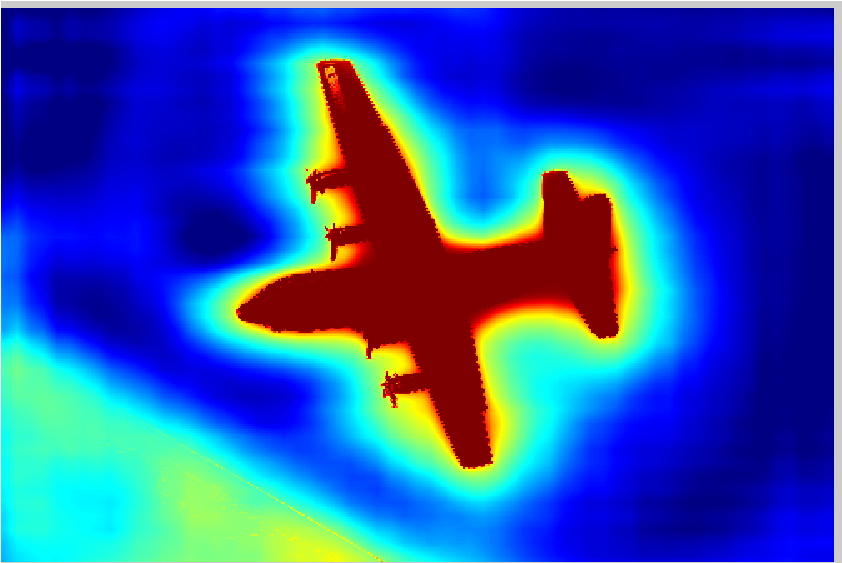
\includegraphics[width=0.16\linewidth]{fig/mean_field_illustration/Score_Class1_Itr2.pdf} & 
    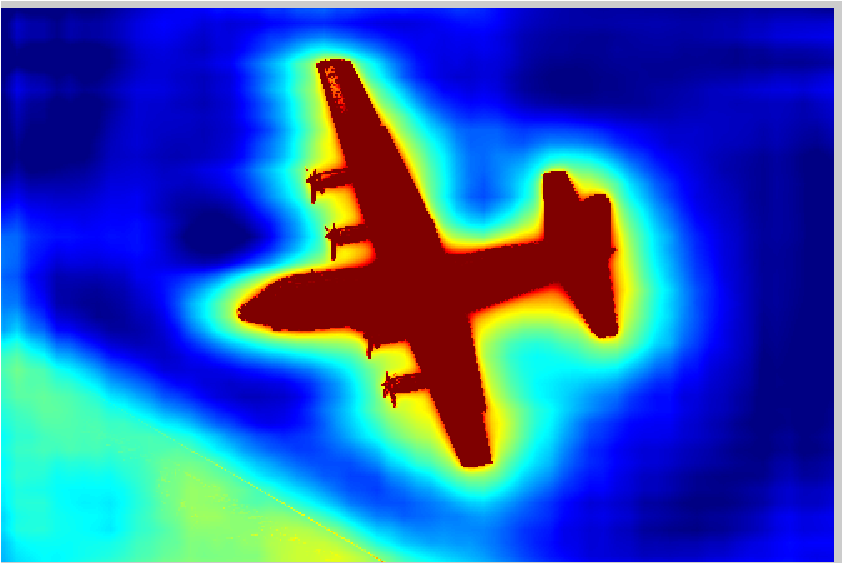
\includegraphics[width=0.16\linewidth]{fig/mean_field_illustration/Score_Class1_Itr10.pdf} \\
    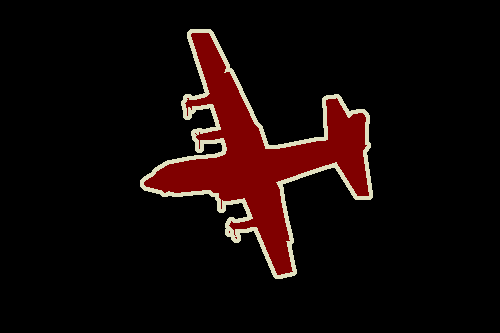
\includegraphics[width=0.16\linewidth]{fig/mean_field_illustration/2007_007470.png} & 
    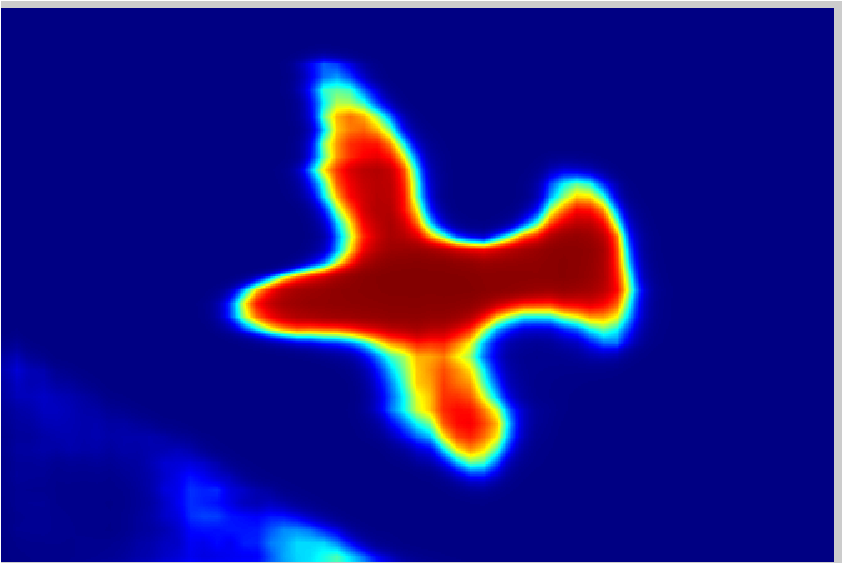
\includegraphics[width=0.16\linewidth]{fig/mean_field_illustration/Belief_Class1_Itr0.pdf} & 
    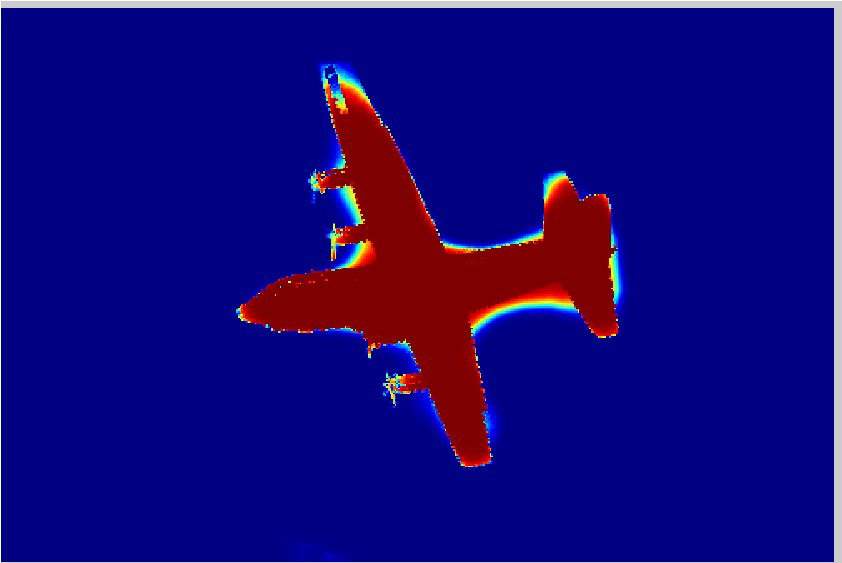
\includegraphics[width=0.16\linewidth]{fig/mean_field_illustration/Belief_Class1_Itr1.pdf} & 
    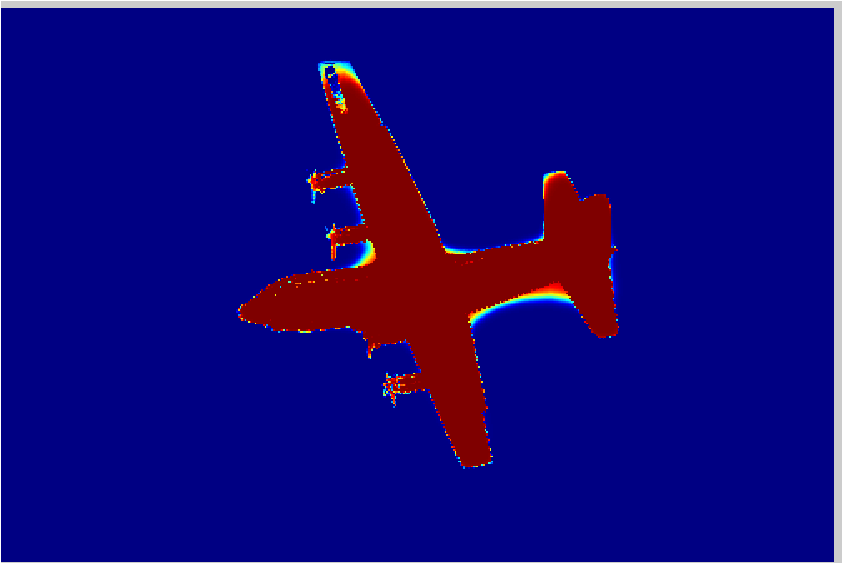
\includegraphics[width=0.16\linewidth]{fig/mean_field_illustration/Belief_Class1_Itr2.pdf} & 
    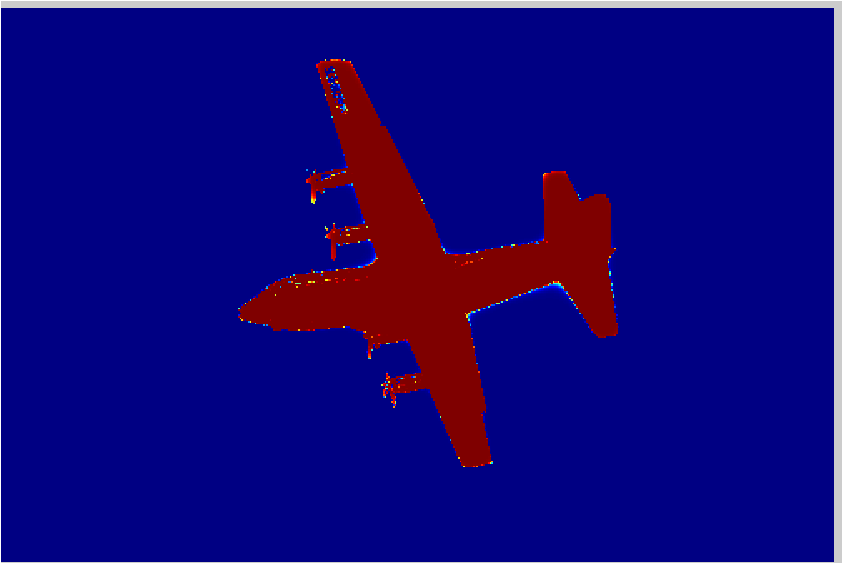
\includegraphics[width=0.16\linewidth]{fig/mean_field_illustration/Belief_Class1_Itr10.pdf} \\
    Image/G.T. & DCNN output & CRF Iteration 1 & CRF Iteration 2 & CRF Iteration 10 \\
  \end{tabular}
  \caption{Score map (input before softmax function) and belief map (output of softmax function) for Aeroplane. We show the score (1st row) and belief (2nd row) maps after each mean field iteration. The output of last DCNN layer is used as input to the mean field inference. Best viewed in color.}
  \label{fig:score-maps}
\end{figure}

Traditionally, conditional random fields (CRFs) have been employed to smooth
noisy segmentation maps \cite{rother2004grabcut, kohli2009robust}. Typically
these models contain energy terms that couple neighboring nodes, favoring
same-label assignments to spatially proximal pixels. Qualitatively, the
primary function of these short-range CRFs has been to clean up the spurious
predictions of weak classifiers built on top of local hand-engineered features.

Compared to these weaker classifiers, modern DCNN architectures such as
the one we use in this work produce score maps and semantic label
predictions which are qualitatively different. As illustrated in
Figure~\ref{fig:score-maps}, the score maps are typically quite smooth and
produce homogeneous classification results. In this regime, using short-range
CRFs can be detrimental, as our goal should be to recover detailed local
structure rather than further smooth it. Using contrast-sensitive potentials
\cite{rother2004grabcut} in conjunction to local-range CRFs can potentially
improve localization but still miss thin-structures and typically requires
solving an expensive discrete optimization problem.

To overcome these limitations of short-range CRFs, we integrate into our system
the fully connected CRF model of \citet{krahenbuhl2011efficient}.
The model employs the energy function
\begin{align}
  E(\boldsymbol{x}) = \sum_i \theta_i(x_i) + \sum_{ij} \theta_{ij}(x_i, x_j)
\end{align}
where $\boldsymbol{x}$ is the label assignment for pixels. We use as unary
potential $\theta_i(x_i) = - \log P(x_i)$, where $P(x_i)$ is the label
assignment probability at pixel $i$ as computed by DCNN. The pairwise
potential is $\theta_{ij}(x_i, x_j) = \mu(x_i,x_j)\sum_{m=1}^{K} w_m \cdot
k^m(\boldsymbol{f}_i, \boldsymbol{f}_j)$, where $\mu(x_i,x_j)=1 \text{ if } x_i \neq x_j$, and zero otherwise (\ie, Potts Model). There is one pairwise term for each
pair of pixels $i$ and $j$ in the image no matter how far from each other they
lie, \ie the model's factor graph is fully connected. Each $k^m$ is the
Gaussian kernel depends on features (denoted as $\boldsymbol{f}$) extracted for pixel $i$ and $j$ and is
weighted by parameter $w_m$. We adopt bilateral position and color terms,
specifically, the kernels are
\begin{align}
  \label{eq:fully_crf}
  w_1 \exp \Big(-\frac{||p_i-p_j||^2}{2\sigma_\alpha^2} -\frac{||I_i-I_j||^2}{2\sigma_\beta^2} \Big) + w_2 \exp \Big(-\frac{||p_i-p_j||^2}{2\sigma_\gamma^2}\Big)
\end{align}
where the first kernel depends on both pixel positions (denoted as $p$) and
pixel color intensities (denoted as $I$), and the second kernel only depends
on pixel positions. The hyper parameters $\sigma_\alpha$, $\sigma_\beta$ and
$\sigma_\gamma$ control the ``scale'' of the Gaussian kernels.

Crucially, this model is amenable to efficient approximate probabilistic
inference \citep{krahenbuhl2011efficient}. The message passing updates under a
fully decomposable mean field approximation $b(\boldsymbol{x}) = \prod_i
b_i(x_i)$ can be expressed as convolutions with a Gaussian kernel in feature
space. High-dimensional filtering algorithms \citep{adams2010fast}
significantly speed-up this computation resulting in an algorithm that is very
fast in practice, less that 0.5 sec on average for Pascal VOC images using the
publicly available implementation of \citep{krahenbuhl2011efficient}.

\begin{figure}
  \centering
  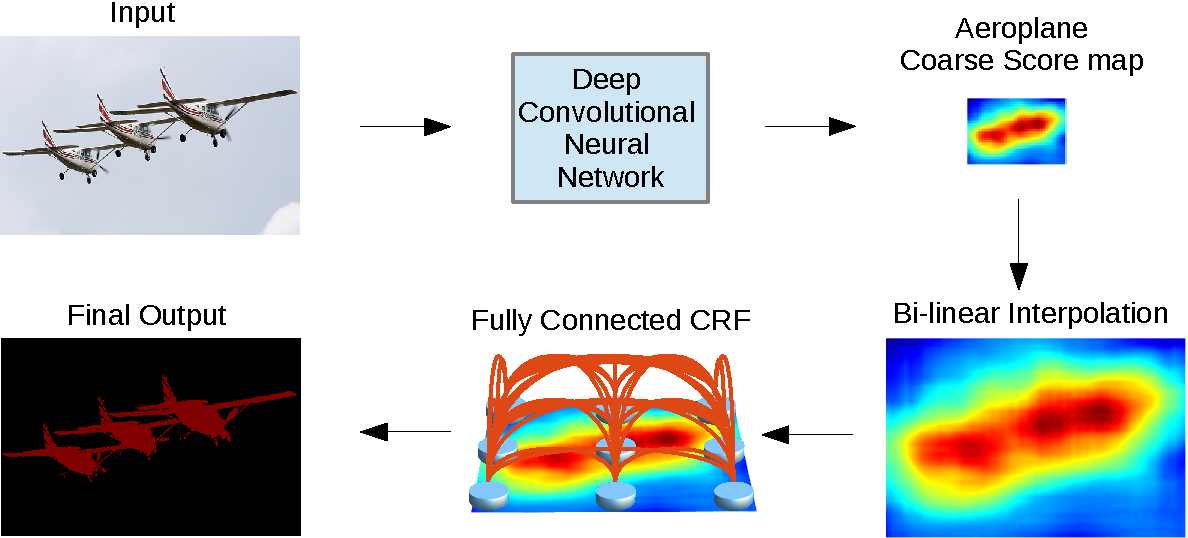
\includegraphics[width=0.7\linewidth]{fig/model_illustration3.pdf}
  \caption{Model Illustration. The coarse score map from Deep Convolutional Neural Network (with fully convolutional layers) is upsampled by bi-linear
    interpolation. A fully connected CRF is applied to refine the segmentation result. Best viewed in color.}
  \label{fig:ModelIllustration}
\end{figure}

\subsection{Multi-Scale Prediction}
\label{sec:multiscale}

Following the promising recent results of \cite{hariharan2014hypercolumns,
  long2014fully} we have also explored a multi-scale prediction method to
increase the boundary localization accuracy. Specifically, we attach to the input image and each of the first four max pooling layers a two-layer MLP (first layer: 128 3x3 convolutional filters, second layer: 128 1x1 convolutional filters) whose score map is concatenated to the VGG final layer score map. The final score map fed into the softmax layer thus consists of 4,096 + 5 * 128 = 4,736 channels. We
only adjust the newly added weights, keeping the other network parameters to
the values learned by the method of Section~\ref{sec:convnets}. As
discussed in the experimental section, introducing these extra direct
connections from fine-resolution layers improves localization performance, yet
the effect is not as dramatic as the one obtained with the fully-connected
CRF. 
